\chapter{Introducción}
\section{Motivación del proyecto}

En el año 1994, tras una reunión en Sillicon Valley, Timothy C. May publica el manifiesto cripto-anarquista \cite{criptoanarquista} que da origen al movimiento Cyberpunk. Este movimiento social es el origen de una revolución de carácter libertaria cuyo principal objetivo es reducir la intervención del Estado a su mínima expresión. Se consideraba que la protección brindada por el Estado en la relación y acuerdos entre individuos, podía ser brindada de una manera más libertaria y eficiente por la tecnología. Dicho movimiento siembra las premisas de un proyecto que surge años después, el proyecto Bitcoin. \newline

El 1 de noviembre de 2008 se publica un \textit{whitepaper} titulado “Bitcoin: A Peer-to-Peer Electronic Cash System” \cite{bitcoin}. El autor (o autores) del \textit{whitepaper}, que se esconde bajo el alias Satoshi Nakamoto, decide publicarlo en una lista de correo sobre criptografía. Este es uno de los primeros documentos en los que se menciona el término Blockchain. Se describe como una tecnología creada con el propósito de llevar a cabo el proyecto de Bitcoin. Blockchain surge de la ingeniosa combinación de distintas técnicas creadas años atrás en el campo de la informática y la criptografía. Apoyándose en los ideales del movimiento Cyberpunk, se describe al Bitcoin como una moneda digital gobernada por unas reglas criptográficas que controlan su gestión y emisión. La tecnología blockchain garantiza el correcto funcionamiento de los aspectos clave de las criptomonedas: la puesta en circulación de la moneda y el mecanismo de gasto que garantiza que una moneda no pueda ser gastada varias veces. Anteriores monedas digitales habían intentado resolver estos dos problemas sin éxito. El proyecto Bitcoin, cuya base tecnológica es blockchain, es la primera criptomoneda capaz de resolverlos de manera totalmente descentralizada. \newline

Como cualquier otra nueva tecnología, Blockchain debe pasar por todas las fases de adopción que se observan en la figura XXXXXXXXXXX. Durante los primero años, el término blockchain está ligado directamente con el proyecto Bitcoin, ambos términos se conciben como un todo. \newline

\begin{figure}
	\centering
	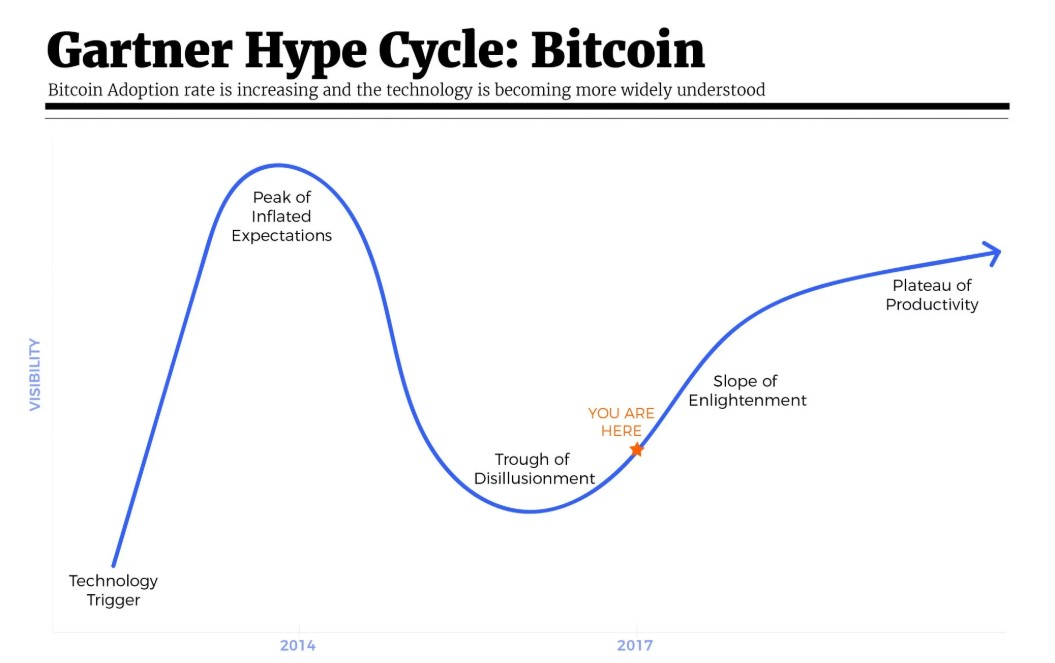
\includegraphics[width=1\textwidth]{imagenes/hypercycle.jpg}
	\caption{\label{fig1}Curva Gartner de Bitcoin \cite{gartner}.}
\end{figure}

El gran abanico de posibilidades que parece ofrecer blockchain a parte de Bitcoin hace que se llegue al pico de expectación de la tecnología. Aunque se empieza a entender que blockchain y Bitcoin no son la misma cosa, el interés por blockchain se sigue manifestando de la manera más accesible por cualquier persona, comprando bitcoin. No se debe confundir la curva de la figura XXXXXX con la del precio de Bitcoin. La fase de desilusión de la tecnología no se corresponde con la bajada de precio de Bitcoin. A medida que se estudia a fondo blockchain y todos sus posibles casos de uso afloran todos los inconvenientes y problemas de la tecnología. El principal problema es la escalabilidad. Este hace que se empiece a pensar que la tecnología que parecía poderse aplicar a un sinfín de usos ahora no se pueda aplicar a nada. En la fase \textit{pendiente de la iluminación} en la que se encuentra blockchain actualmente se tratan de solucionar todos los problemas que se han descubierto en la anterior fase para poder aplicar la tecnología a los sectores en los que de verdad aporta valor. Es así como se consigue llegar a la "meseta de productividad".  





\section{Objetivos}

En el apartado ANTERIORXXXXXXXXXXXXXXXXXXX se describen algunos de los hitos más relevantes del origen de las criptomonedas y blockchain. La actual fase en la que se encuentra la tecnología motiva la realización del presente trabajo. En este apartado se enumerarán los objetivos concretos del trabajo con el que se pretende contribuir a la mejora de la escalabilidad de blockchain. \newline

A continuación se enumeran los objetivos del presente trabajo, partiendo desde los más simples y concretos hasta llegar a los objetivos que constituyan el sistema que se quiere desarrollar:

\begin{enumerate}
	\item Mecanismo con el cuál comparar la sincronización de dos relojes. Para ello se necesita comparar cada reloj por separado con una misma referencia temporal mutua para ambos.
	\item Generación de ficheros RINEX mediante un dispositivo receptor GPS.
	\item A partir de los ficheros RINEX y haciendo uso del software R2CGGTTS generar el fichero con el que obtener la trazabilidad temporal. Al fichero se le denomina CGGTTS.
	\item Estudiar los distintos fabricantes de procesadores que ofrecen Trusted Execution Environment (TEE). A partir del estudio elegir el sistema empotrado que se usará.
	\item Desarrollar una aplicación de ejemplo que se ejecute en uno de estos enclaves seguros de ejecución.
	\item Desarrollar un sistema operativo seguro y confiable que constituya el ambiente de ejecución seguro en el que se ejecutará la aplicación desarrollada.
	\item Ejecución de un protocolo de sincronización de relojes que proporcione precisión al sistema. En concreto PTPd (Precision Time Protocol daemon).
	\item La aplicación será la encargada de realizar el sellado temporal de información. En concreto, realizará el sellado temporal de los \textit{hashes}, los bloques de blockchain y del fichero CGGTTS.
	\item Desarrollar un protocolo blockchain alternativo que haga uso del sistema de sellado temporal confiable.
	\item Evaluación de la mejora de escalabilidad conseguida con el protocolo desarrollado.
\end{enumerate}

Los objetivos que se acaban de enumerar buscan combinar el potencial de dos tecnologías como son la Trazabilidad temporal y los Trusted Execution Environment. Dicha combinación permite sacar más partido de la tecnología blockchain haciéndola más eficiente y escalable.

\section{Materiales y métodos}


Para la realización del presente trabajo se necesitan una serie de materiales (hardware y software) y seguir una serie de metodologías con las que conseguir los objetivos marcados. Se distinguen 3 tipos de objetivos, por lo que cada uno necesitará de sus materiales y métodos\newline

\subsection{Trazabilidad de tiempo}
Para conseguir los objetivos relacionados con la trazabilidad de tiempo se hace uso del siguiente dispositivo y librerías de código.

\subsubsection{Dispositivo U-blox}
La empresa U-blox fabrica una serie de dispositivos de posicionamiento GPS (entre otros propósitos). Haciendo uso de uno de sus dispositivos y del programa u-center se consiguen generar ficheros en formato ublox que contienen los mensajes enviados por los satélites GPS y recibidos por el dispositivo. A partir de dichos ficheros se generan los ficheros RINEX. Para este trabajo se ha hecho uso del dispositivo U-blox EVK-M8F \cite{ublox}.

\subsubsection{RTKLIB}
Se trata de un conjunto de librerías y aplicaciones de código libre destinadas al posicionamiento GNSS. Soporta multitud de dispositivos receptores, formatos, versiones, etc. Las aplicaciones que hacen uso de las librerías permiten entre otras cosas generar ficheros RINEX (GPS, GLONASS, Galileo, ...) a partir de ficheros ublox. Se hace uso de la aplicación CONVBIN que usa la librería RTKCONV \cite{rtklib}.

\subsubsection{R2CGGTTS}
RINEX to CGGTTS es una herramienta software \cite{ftpr2cggtts} creada por el Royal Observatory of Belgium capaz de crear ficheros CGGTTS a partir de ficheros RINEX.

\subsection{Trusted Execution Environment (TEE)}
Para la seguridad y confiabilidad del sistema se necesita un TEE. Varios fabricantes de procesadores ofrecen esta tecnología, cada uno con sus librerías y para sus dispositivos.

\subsubsection{ARM TrustZone}
El fabricante ARM es uno de los que ofrece esta tecnología. ARM la denomina TrustZone \cite{trustzone}. La mayoría de sus familias de procesadores actuales soportan el uso de TrustZone. En función de la familia del procesador se tendrán unas opciones u otras.

\subsubsection{Zedboard}
Zedboard es un kit de desarrollo para desarrolladores interesados en usar Xilinx Zynq-7000 All Programmable SoC \cite{zedboard}. La tarjeta Zedboard contiene un procesador Dual ARM Cortex-A9 MPCore, uno de los que soportan TrustZone. Para el desarrollo en Zedboard se hace uso del software de Xilinx Vivado y de la documentación de Xilinx relacionada con la seguridad de sus tarjetas.

\subsubsection{Raspberry Pi}
Para el presente trabajo se hace uso de Raspberry Pi 3 Modelo B \cite{rpi}. El principal requisito para el trabajo es su procesador. Este modelo de Raspberry monta un Broadcom BCM2837 Cortex-A53 (ARMv8). Dicha familia de ARM soporta TrustZone.

\subsubsection{OP-TEE}
Open Portable Trusted Execution Environment \cite{optee} es un proyecto de código libre que trata de llevar TEE a multitud de dispositivos. Entre los dispositivos a los que lleva TEE está la Raspberry Pi 3.

\subsubsection{Buildroot}
Buildroot es un proyecto de código libre cuyo propósito es generar sistemas Linux para sistemas empotrados de manera simple y customizable. El proyecto OP-TEE hace uso de Buildroot para generar el sistema operativo, por tanto, si se quieren añadir nuevos paquetes que Buildroot no traiga por defecto hay que hacer uso de sus herramientas \cite{buildroot}.

\subsubsection{Precision Time Protocol (PTP)}
Uno de los paquetes que se le puede añadir al sistema operativo gracias a Buildroot es PTPd \cite{ptpd}. PTP daemon es una implementación del protocolo Precision Time Protocol que permite la sincronización precisa de relojes de equipos conectados mediante Ethernet.

\subsection{Protocolo Blockchain}
El objetivo del presente trabajo es aplicar el sistema desarrollado al protocolo de una red blockchain de manera que esto suponga una mejora en escalabilidad o eficiencia.

\subsubsection{Repositorio Bitcoin}
Para este objetivo no se parte de cero, se parte de un código existente al que se le hacen los correspondientes cambios. El código a utilizar es el de Bitcoin \cite{bitcoincode}, sin embargo, se podrían aplicar los mismos cambios al código de otra blockchain basada en prueba de trabajo. \newline


Tras enumerar los materiales y métodos que se utilizan en el presente trabajo, se pretende hacer ver mediante la figura XXXXXXXXXX la relación entre ellas. A priori pueden parecer tecnologías muy dispares, sin embargo, el sistema desarrollado las combina haciendo que tenga sentido su uso conjunto.


\begin{figure}
	\centering
	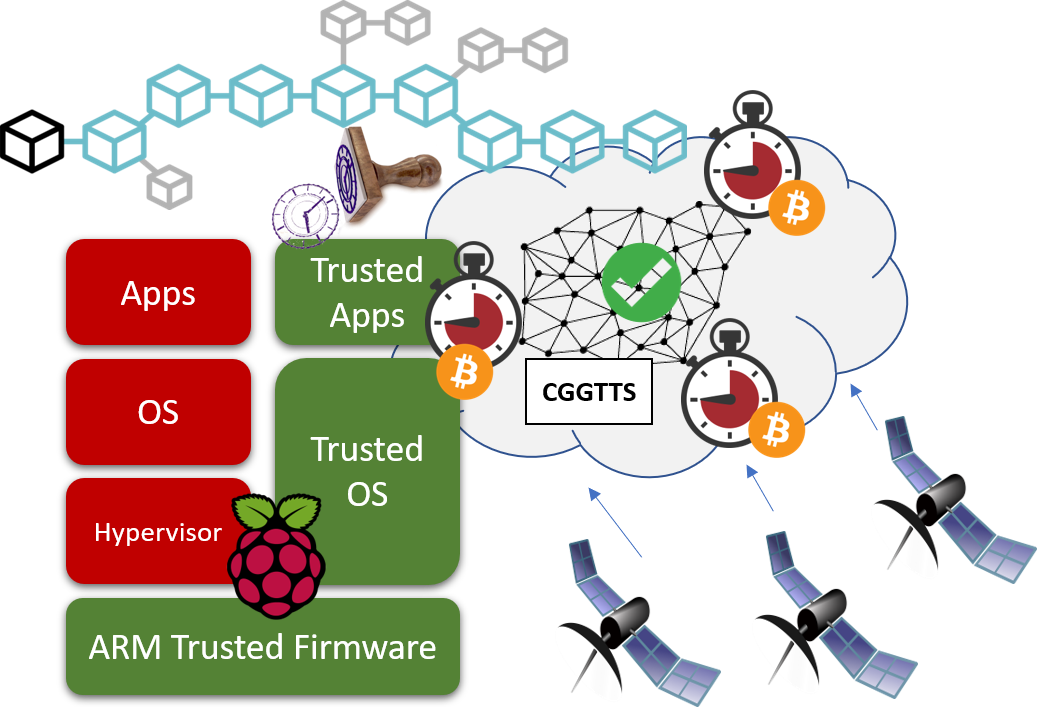
\includegraphics[width=1\textwidth]{imagenes/Imagen2.png}
	\caption{\label{fig1}Combinación de materiales y métodos del trabajo.}
\end{figure}





\section{Organización de la memoria}